%% Copyright (C) 2008 Johan Oudinet <oudinet@lri.fr>
%%
%% Permission is granted to make and distribute verbatim copies of
%% this manual provided the copyright notice and this permission notice
%% are preserved on all copies.
%%
%% Permission is granted to process this file through TeX and print the
%% results, provided the printed document carries copying permission
%% notice identical to this one except for the removal of this paragraph
%% (this paragraph not being relevant to the printed manual).
%%
%% Permission is granted to copy and distribute modified versions of this
%% manual under the conditions for verbatim copying, provided that the
%% entire resulting derived work is distributed under the terms of a
%% permission notice identical to this one.
%%
%% Permission is granted to copy and distribute translations of this manual
%% into another language, under the above conditions for modified versions,
%% except that this permission notice may be stated in a translation
%% approved by the Free Software Foundation
%%
\chapter{Experiments}
Our overall pipeline follows the top-down approach for estimating multiple human poses.
Firstly, we apply a stateof-art bounding detector to generate human proposals.
For each proposal, we assume that there is only one main person in the cropped region of proposal and then applied the pose estimating network to generate the final prediction.
In this chapter, I will discuss more details of our methods based on experiment results.

\section{Experimental Setup}

\subsection{Cropping Strategy}
For each human detection box, the box is extended to a fixed aspect ratio, e.g., height : width = 256 : 192, and then we crop from images without distorting
the images aspect ratio.
Finally, we resize the cropped image to a fixed size of height 384 pixels and width 288 pixels by default.

\subsection{Data Augmentation Strategy}
Data augmentation is critical for the learning of scale invariance and rotation invariance.
After cropping from images, if one case has more than 8 visible keypoint, we apply demi part augmentation with a probability of 0.3.
Then we apply random flip, random rotation $(−45^{\circ} \sim +45^{\circ})$ and random scale $(0.7 \sim 1.35)$.

\subsection{Training Details}
All models of pose estimation are trained using adam algorithm with an initial learning rate of 5e-4.
We train the model for 400 epochs and each epoch contains 90000 samples.
Note that we decrease the learning rate linearly decrease during the whole training process.
We use a weight decay of 1e5 and the training batch size is 32.
Batch normalization is used in our network.
Generally, the training of 4 ResNet-50-based models takes about 5 days on eight NVIDIA Titan X Pascal GPUs.

\subsection{Testing Details}
In order to minimize the variance of prediction, we apply a gaussian filter on the predicted heatmaps.
Following the same techniques used in \cite{newell2016stacked}, we also predict the pose of the corresponding flipped image and average the heatmaps to get the final prediction; a quarter
offset in the direction from the highest response to the second
highest response is used to obtain the final location of
the keypoints.
Rescoring strategy is also used in our experiments.
Different from the rescoring strategy used in \cite{papandreou2017towards},
the product of boxes’ score and the average score of all keypoints
is considered as the final pose score of a person instance.

\section{Ablation Experiment}
In this section, I will validate the effectiveness of our
network from various aspects. Unless otherwise specified,
all experiments are evaluated on MS COCO minival dataset
in this section. The input size of all models is 256×192
and the same data augmentation is adopted.

\subsection{Multi-stage}
A single stage with Res50 is adopted as our baseline. From Table 3, there exists a trade-off between the number of stage and the complexity of one stage because of the computation resource.
Finally, we find 4xres50 is the best choice.  Note that 4xres50 is used in all the next experiments.

\captionsetup[table]{labelformat=empty}
\begin{table}[!hbp]
  \centering
  \begin{tabular}{|c|c|c|c|c|c|c|c|}
  \hline
            & baseline & 2xres50 & 3xres50 & 4xres50 & 2xres101 & 2xresInc101 & 5xres38 \\
  \hline
  AP(OKS) & 73.3 & 76.6 & 77.3 & 77.8 & 77.0 & 77.5 & 77.5 \\
  \hline
  \end{tabular}
  \caption{Table 3: experiments results for multi-stage.}
\end{table}

\subsection{Online Hard Keypoints Mining}
Here I discuss the losses used in our network. In detail,
the loss function of single stage is L2 loss of all annotated
keypoints while the Conv2 tries learning the hard keypoints,
that is, we only punish the top M(M < N) keypoint
losses out of N (the number of annotated keypoints in one
person, say 17 in COCO dataset). The effect of M is shown
in Table 4. For M = 8, the performance of second stage
achieves the best result for the balanced training between
hard keypoints and simple keypoints.

\captionsetup[table]{labelformat=empty}
\begin{table}[!hbp]
  \centering
  \begin{tabular}{|c|c|c|c|c|c|c|}
  \hline
  M          & 6 & 8 & 10 & 12 & 14 & 17 \\
  \hline
  AP(OKS) & 77.4 & 77.8 & 77.5 & 77.5 & 77.1 & 77.0 \\
  \hline
  \end{tabular}
  \caption{Table 4: Comparison of different hard keypoints number in online hard keypoints mining.}
\end{table}

\subsection{Data Pre-processing}
The size of cropped image is a important factor to the performance
of keypoints detection. As Table 5 illustrates, it’s
worth noting that the input size 256×192 actually works as
well as 256×256 which costs more computations of almost
2G FLOPs using the same cropping strategy.
As the input size of the cropped images increases, more location details
of human keypoints are fed into the network resulting in a
large performance improvement.
Additionally, online hard
keypoints mining works better when the input size of the
crop images is enlarged by improving 1 point on 384 × 288
input size.

\captionsetup[table]{labelformat=empty}
\begin{table}[!hbp]
  \centering
  \begin{tabular}{|c|c|c|}
  \hline
  Models          & Input Size & AP(OKS)   \\
  \hline
  4res50* & 256x192 & 76.2 \\
  \hline
  4res50 & 256x192 & 76.9  \\
  \hline
  4res50* & 384x288 & 77.4  \\
  \hline
  4res50 & 384x288 & 77.8  \\
  \hline
  \end{tabular}
  \caption{Table 5: Comparison of models of different input size. 4xres50* indicates 4xres50 without online hard keypoints mining.}
\end{table}

\subsection{Ensemble on Heatmap}

At the end, we use ensemble on the heatmap level to get the best results.

\captionsetup[table]{labelformat=empty}
\begin{table}[!hbp]
  \centering
  \begin{tabular}{|c|c|c|c|}
  \hline
  Models          & AP-minival & AP-dev & AP-challenge  \\
  \hline
  4res50 & 77.8 & 74  & - \\
  \hline
  4res50+ & 80 & 77.8 & 76.2  \\
  \hline
  \end{tabular}
  \caption{Table 6: Comparison of results on the minvival dataset and the corresponding results on test-dev or test-challenge of the COCO
dataset. “+” indicates ensembled model.}
\end{table}

\captionsetup[figure]{labelformat=empty}
\begin{figure}[htbp]
  \centering
  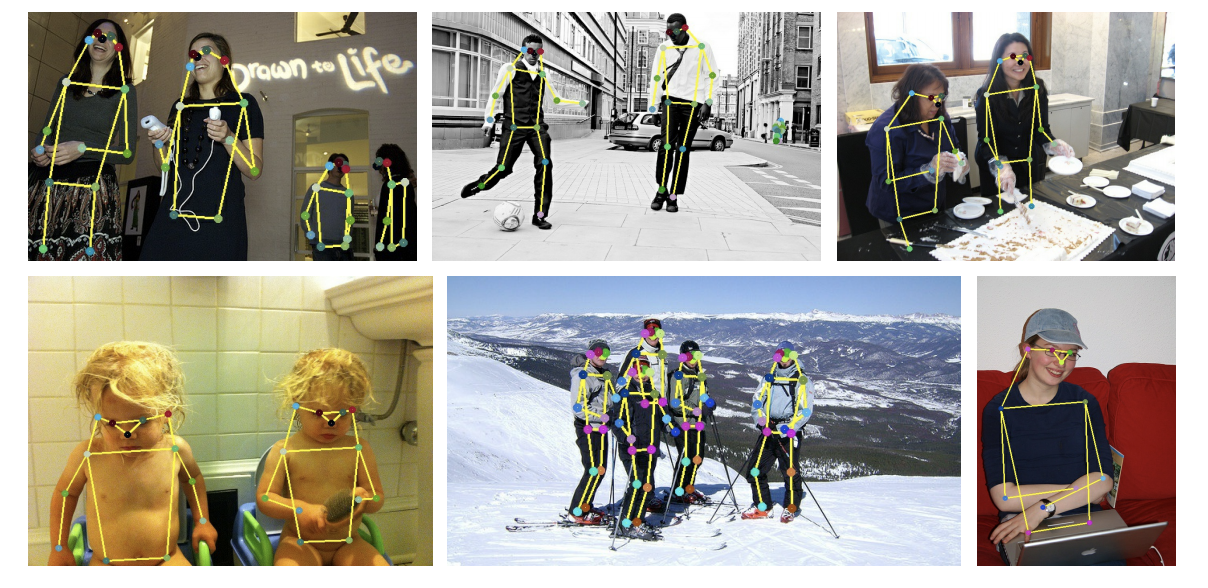
\includegraphics[width=16cm,height=8cm]{source/result.png}
  \caption{Figure 9: Some results of our method.}
\end{figure}






%%% Local Variables:
%%% mode: latex
%%% TeX-master: "rapportM2R"
%%% End:
